\documentclass[11pt,bibliography=totoc]{scrartcl}

% Son titrage
\author{Juan-Carlos Barros et Daniel Kessler}
\date{\today}
\title{Conception d'une séquence d'enseignement\\\medskip
  \large GymInf, Didactique de l'informatique, Rendu 010}

% son français
\usepackage[french]{babel}
\usepackage{csquotes}

% Sa gestion de bibliographie
% NB: nos consignes nous demandent d'utiliser les normes APA
%     ça tombe bien, c'est possible de le préciser ici!
\usepackage[backend=biber,style=apa,
            urldate=edtf,date=edtf,seconds=true]{biblatex}
\addbibresource{biblio.bib}

% configuration générale
\usepackage[l2tabu, orthodox]{nag}  % demander indication d'usages désuets
\usepackage{microtype}  % subtiles améliorations de certains défauts
\usepackage[french]{babel}  % langue du document
\usepackage{graphicx}  % pour inclure des images et des pdf

% configuration des polices de caractère / aspect du titre
\usepackage[utf8]{inputenc}  % nécessaire en MS-Windows, pas dans Linux
                             % (probablement pas dans MacOS non plus)
% Possibles changements de police ci-dessous (en décomenter un, ou pas)
\usepackage[T1]{fontenc}  % <- c'est nécessaire dans window$, je crois
% \usepackage{tgtermes} %  (semble nécessiter lualatex)

% pdfisation avec liens un peu bleus mais pas trop
\usepackage[pdfstartview=FitH,
pdfauthor={Juan-Carlos Barros et Daniel Kessler},
pdftitle={Conception d'une séquence}]{hyperref}
\usepackage{xcolor}
\definecolor{pdflinkcolor}{RGB}{30,60, 120}
\hypersetup{colorlinks=true, allcolors=pdflinkcolor}

\begin{document}

% Démarrage avec titre et table des matières sur page séparée
\maketitle
\tableofcontents  % <- au début, on n'est pas des frouzes qui mettent ça à la fin...
\pagebreak

% Et c'est parti pour du contenu!
\section{Contexte institutionnel et disciplinaire}
Nous enseignons tous deux au niveau gymnasial dans le Collège de Genève. Dans ce
cadred, nous avons cette année plusieurs groupes d'élèves de 1ère année
informatique discipline fondamentale, auxquels s'adresse le travail présenté
dans ce document. Ces groupes sont constitués de 16 élèves, issus
potentiellement de plusieurs ``classes'' (le concept de ``classe'' est très flou
au Collège, les élèves changeant souvent de groupe pour des matières à effectif
réduit, selon leur niveau de maths, leurs choix d'options, etc.).

La séquence d'enseignement que nous allons présenter possède deux
caractéristiques distinctives:
\begin{itemize}
\item Elle se déroule sur plusieurs leçons, en prenant 20-30 minutes du cours à
  chaque fois.
\item Elle combine des objectifs explicites pour les élèves avec des objectifs
  implicites qui seront explicités plus tard.
\end{itemize}

Cette séquence s'insère en deuxième partie du premier semestre, après avoir
travaillé sur le code binaire, vu quelques encodages simples (nombres entiers,
caractères \textsc{ascii}, bitmaps) et travaillé un petit peu sur les composants
matériels d'un ordinateur, éléments du chapitre \textit{Information et Données}
du plan d'étude cantonal genevois \autocite{pecinfo}.

L'objectif explicite initial de la séquence présentée dans ce document est
d'approfondir un des éléments précédents, à travers un travail de groupe sur un
sujet qui n'a été qu'effleuré pendant la première partie de l'année scolaire
(par exemple l'encodage des nombres à virgule flottante, la parenté entre les
composants d'un smartphone et ceux d'un PC, etc.)

Le deuxième objectif, initialement implicite, est de comprendre comment
fonctionne un \textit{wiki} en en utilisant un comme outil, pour découvrir
finalement que certains wikis sont très ouverts aux contributions publiques,
notamment \textit{Wikipedia}. Après avoir expérimenté le travail sur un wiki, un
élève devrait comprendre le mécanisme de base et se sentir capable de contribuer
à Wikipedia s'il ou elle y repère une coquille à corriger, une information
caduque ou incomplète, etc. Ce deuxième objectif participe à plusieurs thèmes du
plan d'étude notamment les \textit{Réseaux}, \textit{Information et Données} et
la \textit{Citoyenneté Numérique}.

\section{Objectifs pédagogiques}
La majorité de cette séquence se déroule en suivant le paradigme
\textit{socio-constructiviste} [citer un article ici]. En effet, les élèves
contruisent une partie de leur propre connaissance en effectuant leurs propres
recherches et en collaborant avec leurs camarades.

bla bla en plus, notamment sur le rôle du prof

Cependant, cela n'empêche pas quelques moments ``frontaux'', notamment bla bla 

\section{Scénario d'apprentissage}
Nous pouvons découper le scénario d'apprentissage en cinq étapes, en suivant le
modèle de Robert Bibeau \autocite{bibeau}.

\subsection{Mise en situation}
bla bla initial et se référer à l'Annexe 1

\subsection{Situation d'apprentissage}
Les élèves ont accès assez vite à une version en-ligne du calendrier suivant des
objectifs minimaux à atteindre chaque semaine. Ce calendrier peut être adapté
suivant les éventuels imprévus.
\begin{center}
\begin{tabular}{rp{.7\textwidth}}
  semaine 1& les groupes et les sujets sont définis\\
  semaine 2& le wiki du groupe a au moins 2 pages différentes et 3 liens
              externes vers des sources;
              la répartition des tâches au sein du groupe (qui fait quoi) est claire et documentée\\
  semaine 3& toutes les informations utiles ont été trouvées et répertoriées
              (liens vers sources);
              un élève d'un autre groupe devrait pouvoir bien comprendre le sujet grâce à ce wiki\\
  semaine 4& chaque élève a lu le wiki d'un autre groupe et fourni des commentaires utiles à celui-ci\\
  semaine 5& le wiki est fini et complet, en prenant en compte les remarques des
             camarades d'autres groupes qui l'ont lu\\
  semaine 6& présentation orale (10 min) avec support à choix (le wiki lui-même ou autre)
\end{tabular}  
\end{center}


\subsection{Objectivation}
ce sera l'évaluation par les pairs des wikis des uns des autres

\subsection{Situation d'évaluation}
L'évaluation de cette séquence prend en compte trois groupes de critères distincts:
\begin{itemize}
\item l'atteinte des objectifs minimaux à la fin de chaque semaine
\item le wiki ``finalisé'' (entre guillemets parce qu'il peut encore être édité
  après: c'est bien le but!)
\item la présentation orale
\end{itemize}
Le détail des critères se trouve dans l'Annexe 2. Il est modelé partiellement
sur les critères d'évaluation officiels du Travail de Maturité. D'ailleurs, le
mode de travail et d'évaluation devrait permettre aussi de donner aux élèves de
1re année un avant-goût d'un TM de type ``travail de recherche'' dans un domaine
scientifique (ce qui peut être explicité à la fin).

\subsection{Situation de réinvestissement}
son wikipedia!

\section{Courant et stratégie pédagogiques}

Une bonne part de la séquence proposée est appelée à se dérouler sous forme de
«petites équipes pour permettre l'apprentissage par les pairs et la
collaboration», ce qui d'après Kozanitis \cite{kozanitis} correspond au modèle
socio-constructiviste. Kozanitis rappelle par ailleurs que dans ce modèle
didactique, «l'enseignant doit veiller en permanence les productions de
l'étudiant et ses process d'apprentissage».

[à élaborer]

\section{Difficultés attendues et problèmes potentiels}

\section{Motivation des élèves et valeurs personnelles}
Comme l'indique Duplessis \cite{duplessis}, nous pouvons nous attendre à des
\textit{a priori} des élèves «sur le monde en général et les objets d'étude en
particulier». En ce qui nous concerne, nous nous attendons à ce qu'ils
s'imaginent que le savoir appris à l'école en général et Wikipedia en
particulier sont des sources de connaissance les élèves ne sont ni auteurs ni
acteurs. Duplessis nous indique qu'«apprendre nécessite que ces conceptions
soient progressivement transformées». Nous espérons qu'à travers le scénario
d'apprentissage proposé, l'élève devienne plus ``acteur'' de son acquisition de
connaissance, et que le futur citoyen aie conscience qu'il peut aussi contribuer
à la connaissance générale au moyen de media collaboratifs comme Wikipedia.
De plus, un ``objectif caché'' lié à nos valeurs personnelles est de faire
découvrir la force du logiciel libre et du \textit{open content} à nos élèves,
sans en faire pour autant un exposé théorique.
 
Nous espérons aussi que le mode de travail sera motivant pour les élèves. Viau
\cite{viau} argumente que l'«apprentissage par projet est l'activité
d'apprentissage qui est perçue par les étudiants comme la plus utile, dans
laquelle ils se sentent le plus compétents et sur laquelle ils ont le sentiment
d'avoir le plus de contrôle». D'après Rolland Viau, ces sentiments de
\textit{compétence} et \textit{contrôle} sont fondamentaux pour que l'élève se
sente bien dans son rôle et puisse ainsi être efficace dans son apprentissage.
En l'occurrence, le contrôle est justement intrinsèquement lié au travail avec
des outils \textit{ouverts}, tels que l'encyclopédie en-ligne Wikipedia: on
n'est pas juste utilisateur, on peut apporter sa petite contribution à l'outil.

L'apprentissage de la Science Informatique devrait aller de pair avec un
changement du regard sur le monde. Jean-Pierre Astolfi \cite{astolfi} considère
justement qu'une discipline «ne se définit pas d'abord par les objets de son
domaine empirique, mais par le type de cardage théorique original que produisent
les concepts» et qu'elle «n'est pas une accumulation de données [...] mais
l'entrée dans une interprétation experte du monde, plus puissante que celle du
sens commun».

% On finit avec sa bibliographie, son colophon et ses annexes
\printbibliography  % pas numéroté, automatiquement au toc
\vfill
% ça c'est un colophon:
\emph{Document réalisé en \href{https://www.latex-project.org/}{\LaTeX}}

% et puis on inclut des annexes
\section*{Annexe 1: définition des groupes et du projet} % pas numéroté, pas au toc
\addcontentsline{toc}{section}{Annexes: supports de cours}  % ajouter au toc
                                % (une entrée pour tous les annexes)
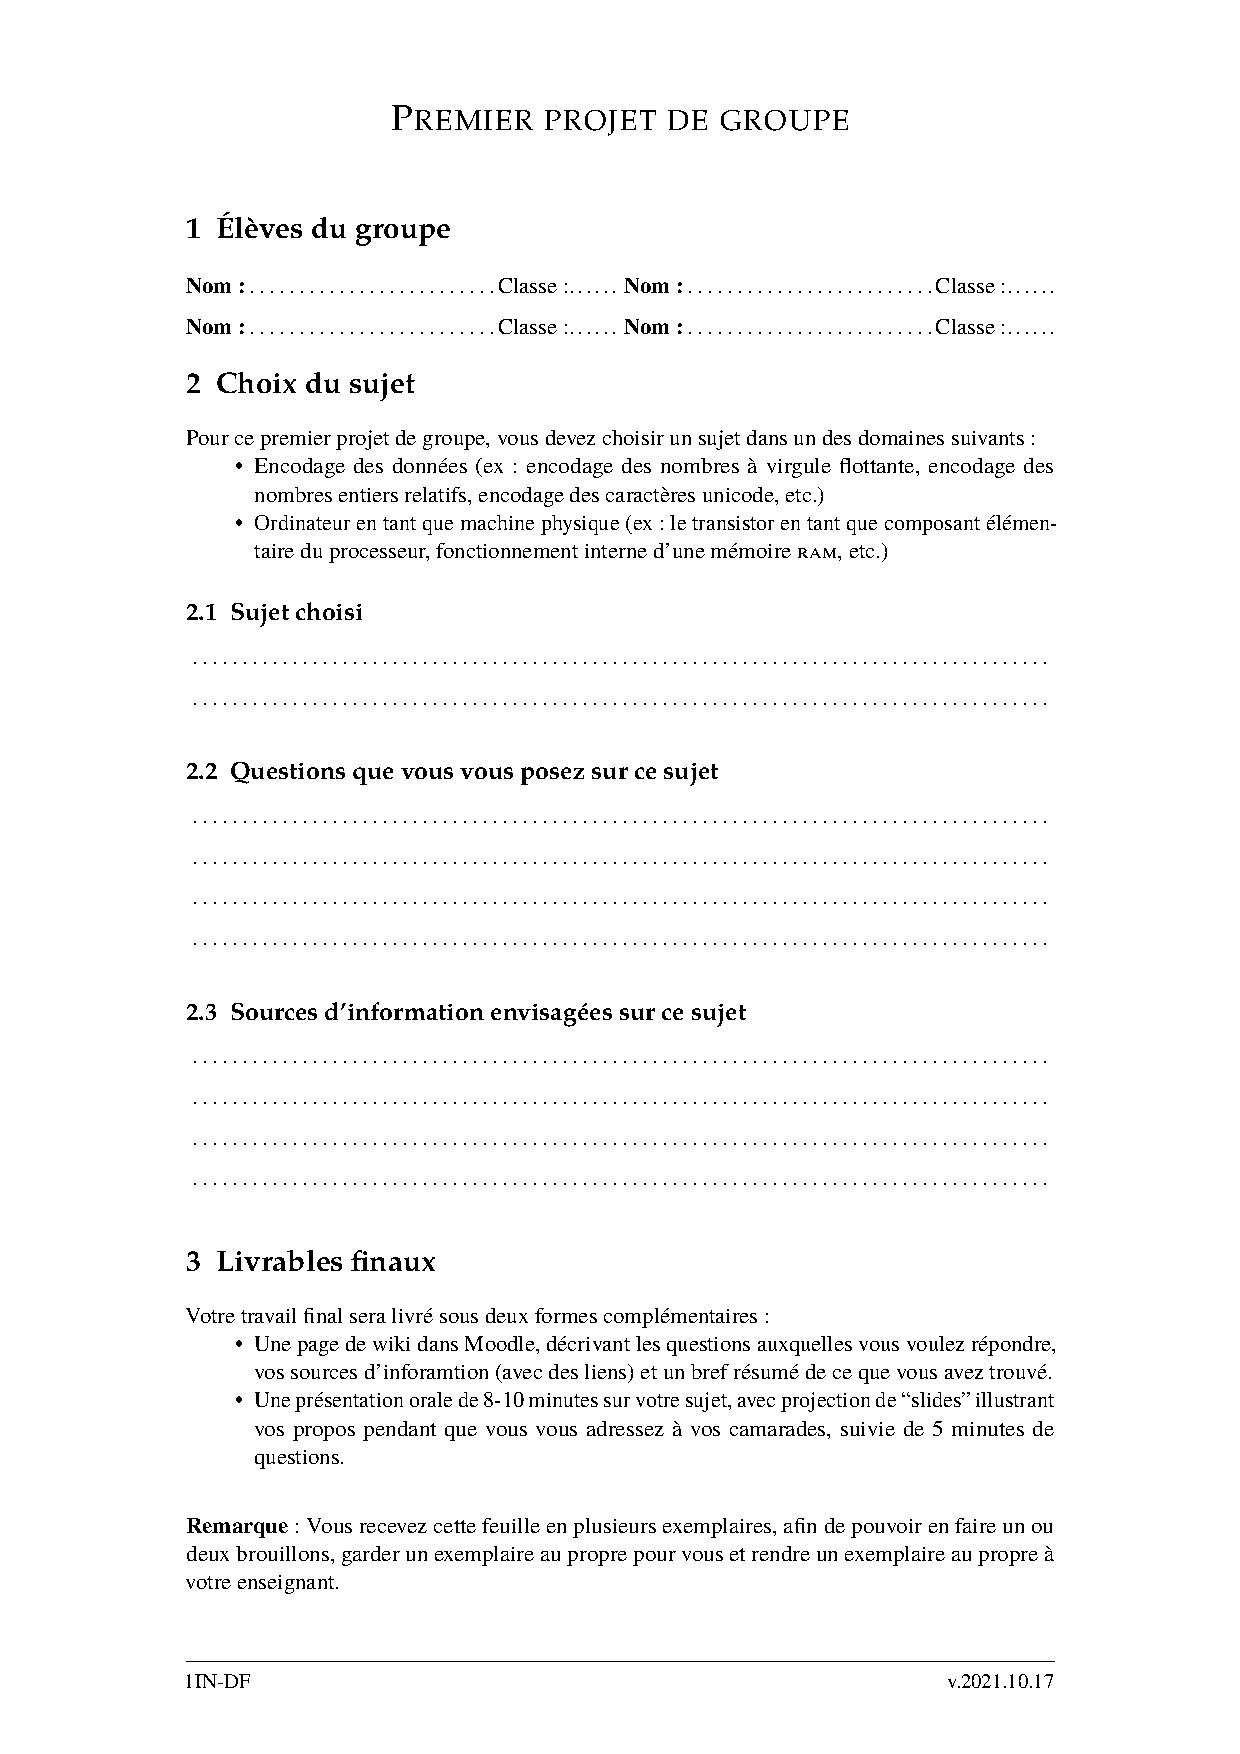
\includegraphics[width=.95\textwidth]{projet1.pdf}

\section*{Annexe 2: grille d'évaluation du projet} % pas numéroté, pas au toc
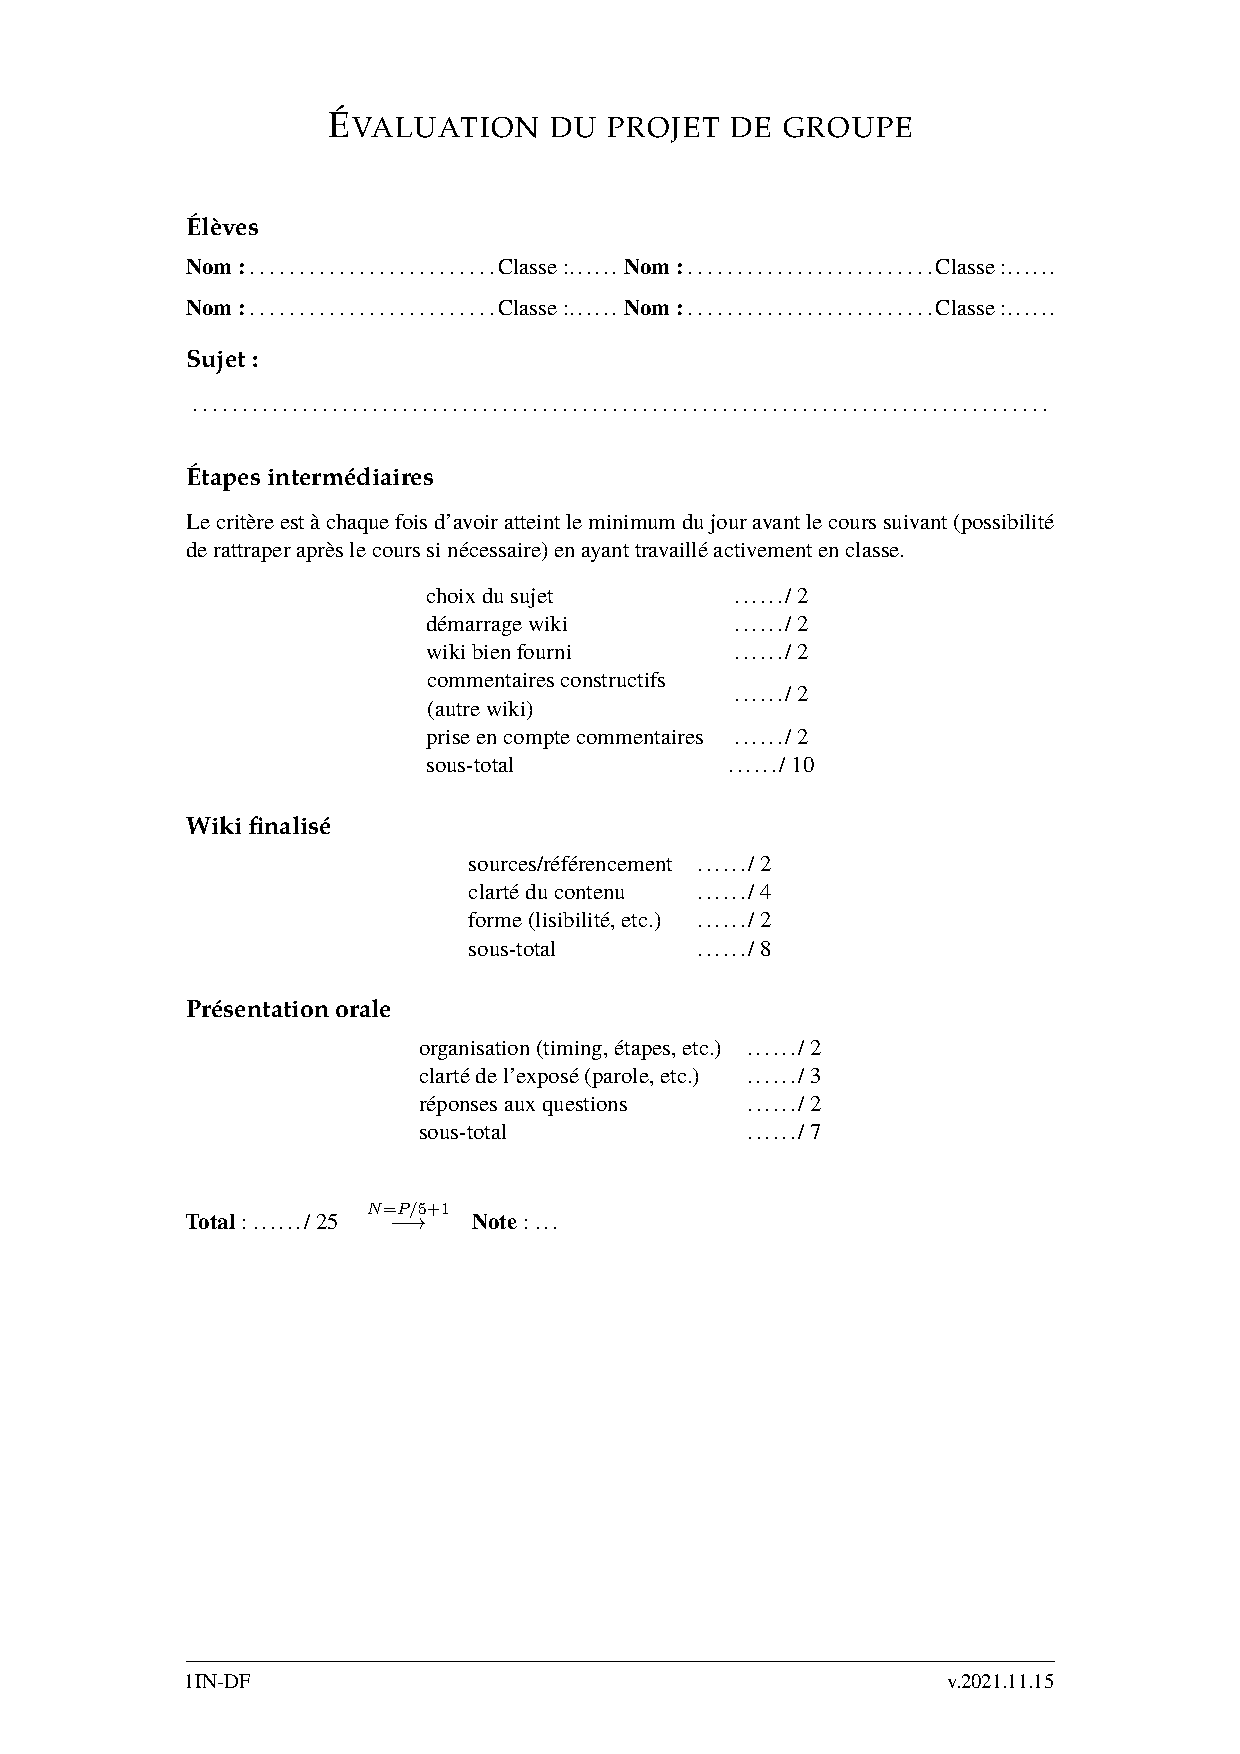
\includegraphics[width=.95\textwidth]{evaluation.pdf}


\end{document}